\ChapterImageStar[cap:disenio]{Diseño de la solución}{./images/fondo.png}\label{cap:disenio}
\mbox{}\\
\section{Modelado del sistema en Archimate}
ArchiMate es un lenguaje de modelado estandarizado por~\textit{The Open Group} que permite representar de manera estructurada y clara las diferentes capas de una arquitectura empresarial: negocio, aplicación y tecnología. Su propósito es brindar una visión integrada que facilite la comunicación entre los distintos actores de un proyecto y que muestre cómo los procesos de negocio, los sistemas de información y la infraestructura tecnológica se relacionan entre sí.
En particular, ArchiMate se organiza en vistas que permiten enfocarse en aspectos específicos: la vista de negocio describe los procesos y actores implicados, la vista de aplicación se centra en los sistemas de software que apoyan esos procesos, y la vista de tecnología aborda la infraestructura que soporta todo el ecosistema. Gracias a este enfoque por capas, los diagramas ayudan a identificar dependencias, puntos de optimización y la coherencia general de la solución arquitectónica.

\subsection{Vista de negocio}
El diagrama~\ref{fig:vista-cooperacion-actores} representa a los distintos actores involucrados en el sistema, como estudiantes, administrativos, docentes y el propio grupo de investigación \GRID. El diagrama muestra cómo se comunican entre sí y cómo intercambian información, destacando elementos como cursos, programas, relaciones contractuales y archivos. En esencia, este diagrama ilustra las interacciones humanas y organizacionales necesarias para el funcionamiento del sistema.

\begin{figure}[H]
    \centering
    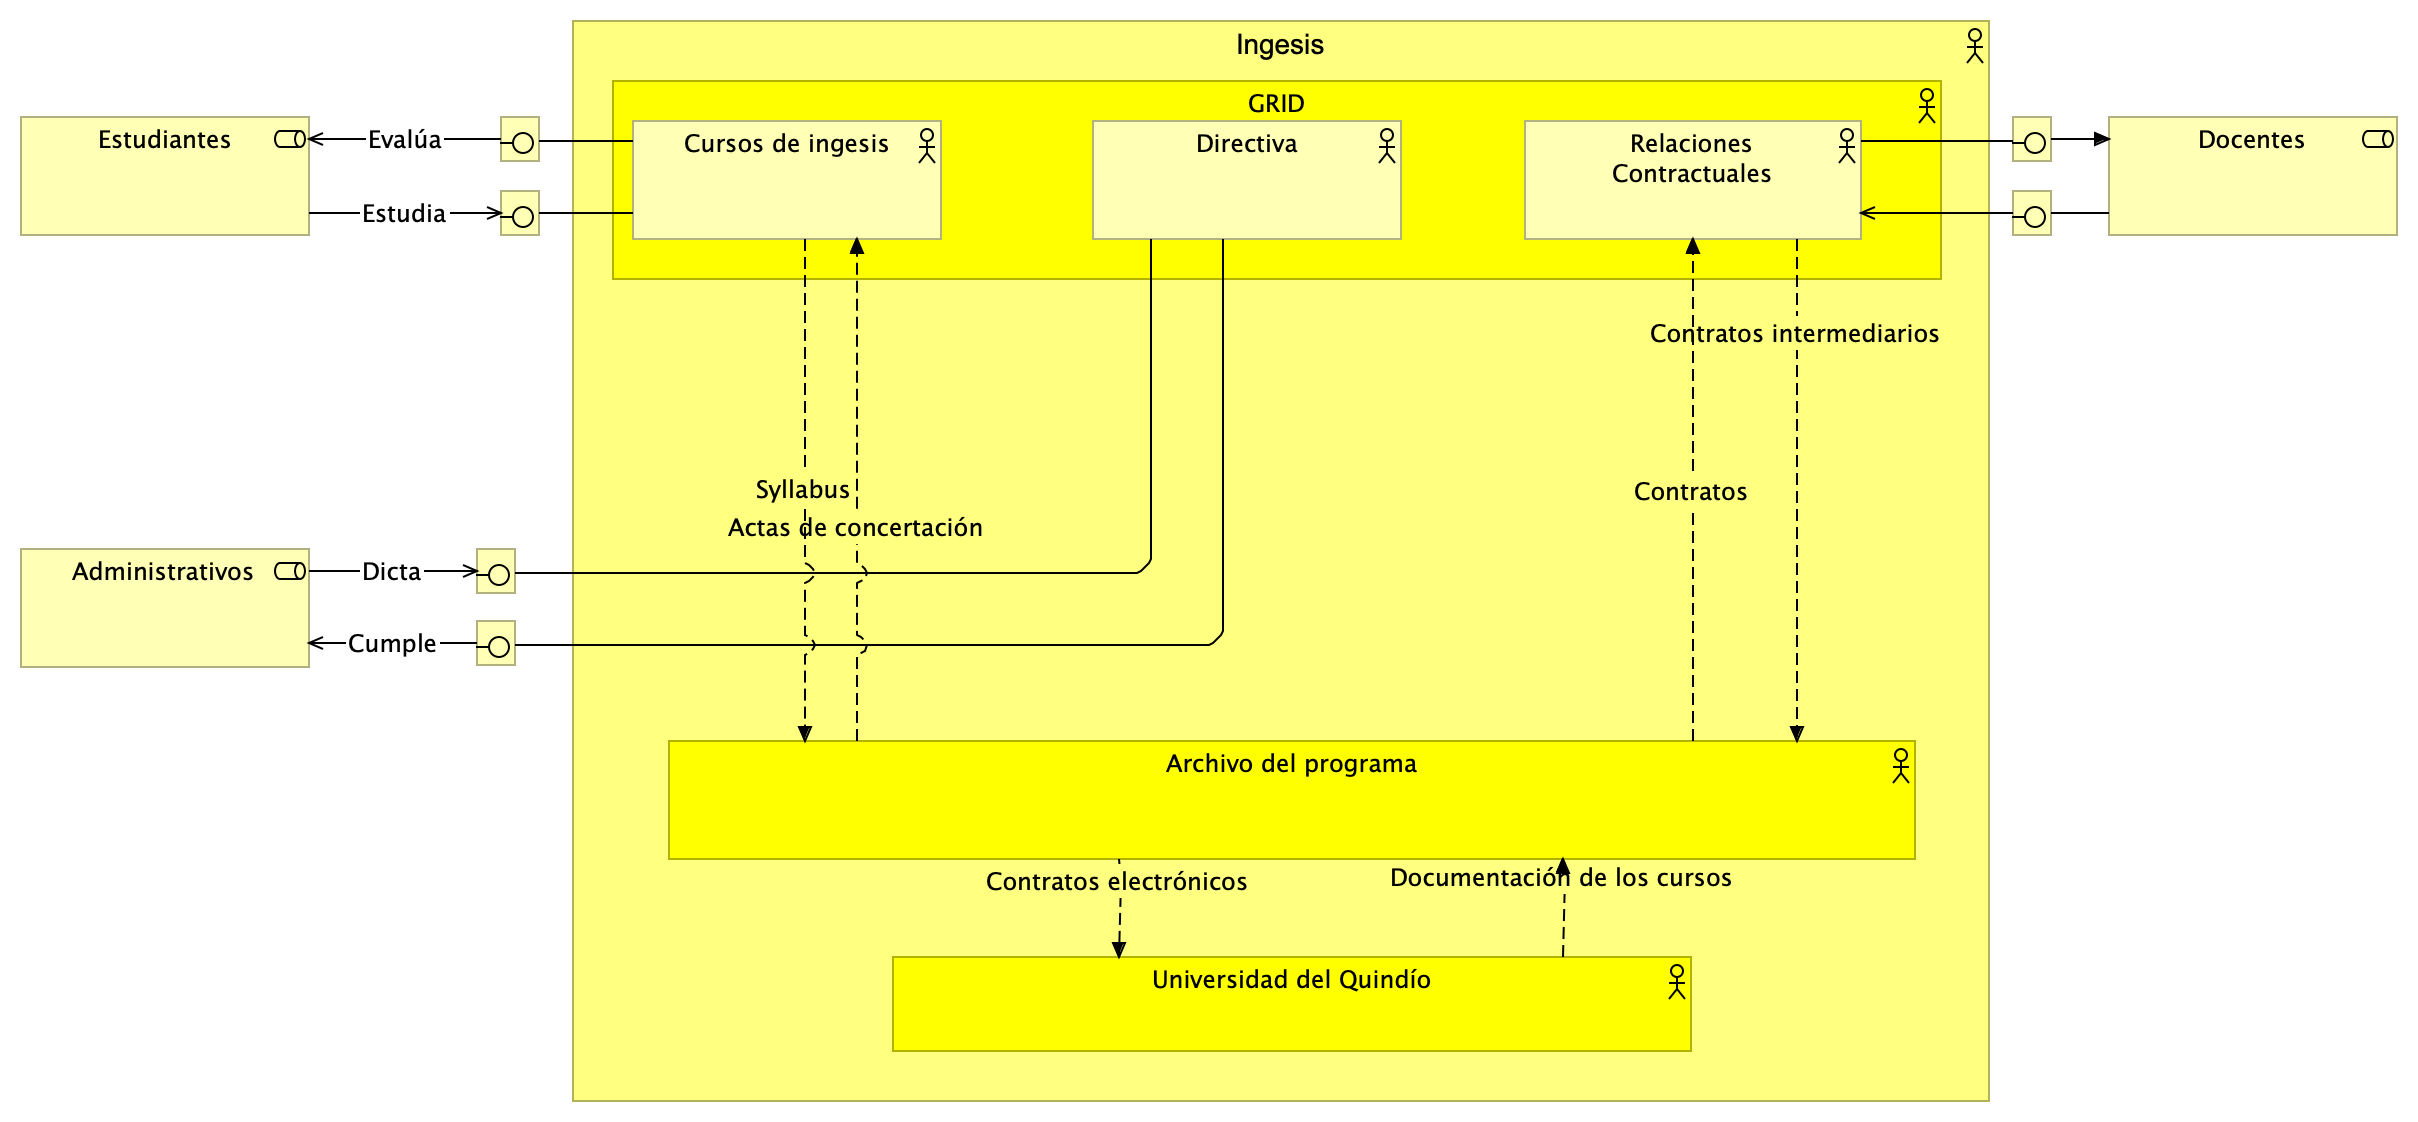
\includegraphics[scale=0.16]{tablas-images/cp6/Actor-Cooperation-view.png}
    \caption{Vista de Cooperación de Actores}\label{fig:vista-cooperacion-actores}
\end{figure}
\noindent
La figura~\ref{fig:vista-cooperacion-negocio} describe los procesos que permiten atender solicitudes de recursos tecnológicos. Estas solicitudes de recursos son descritos en archivos \texttt{.yml}, un ejemplo de solicitud puede verse en el apéndice~\ref{apendice:solicitud-recursos-yaml}, como contenedores, servicios o ingresos. Se observa cómo el investigador o grupo \GRID\ registra una solicitud, pasa por validaciones, asignación de recursos (\CPU, \RAM, \GPU\ y almacenamiento) y finalmente se despliega el contenedor. También se contempla la liberación de recursos cuando dejan de usarse. El diagrama integra servicios como autenticación, orquestación de contenedores y repositorios de imágenes, evidenciando cómo se coordinan los distintos procesos de negocio buscando el cumplimiento de objetivos misionales.

\begin{figure}[H]
    \centering
    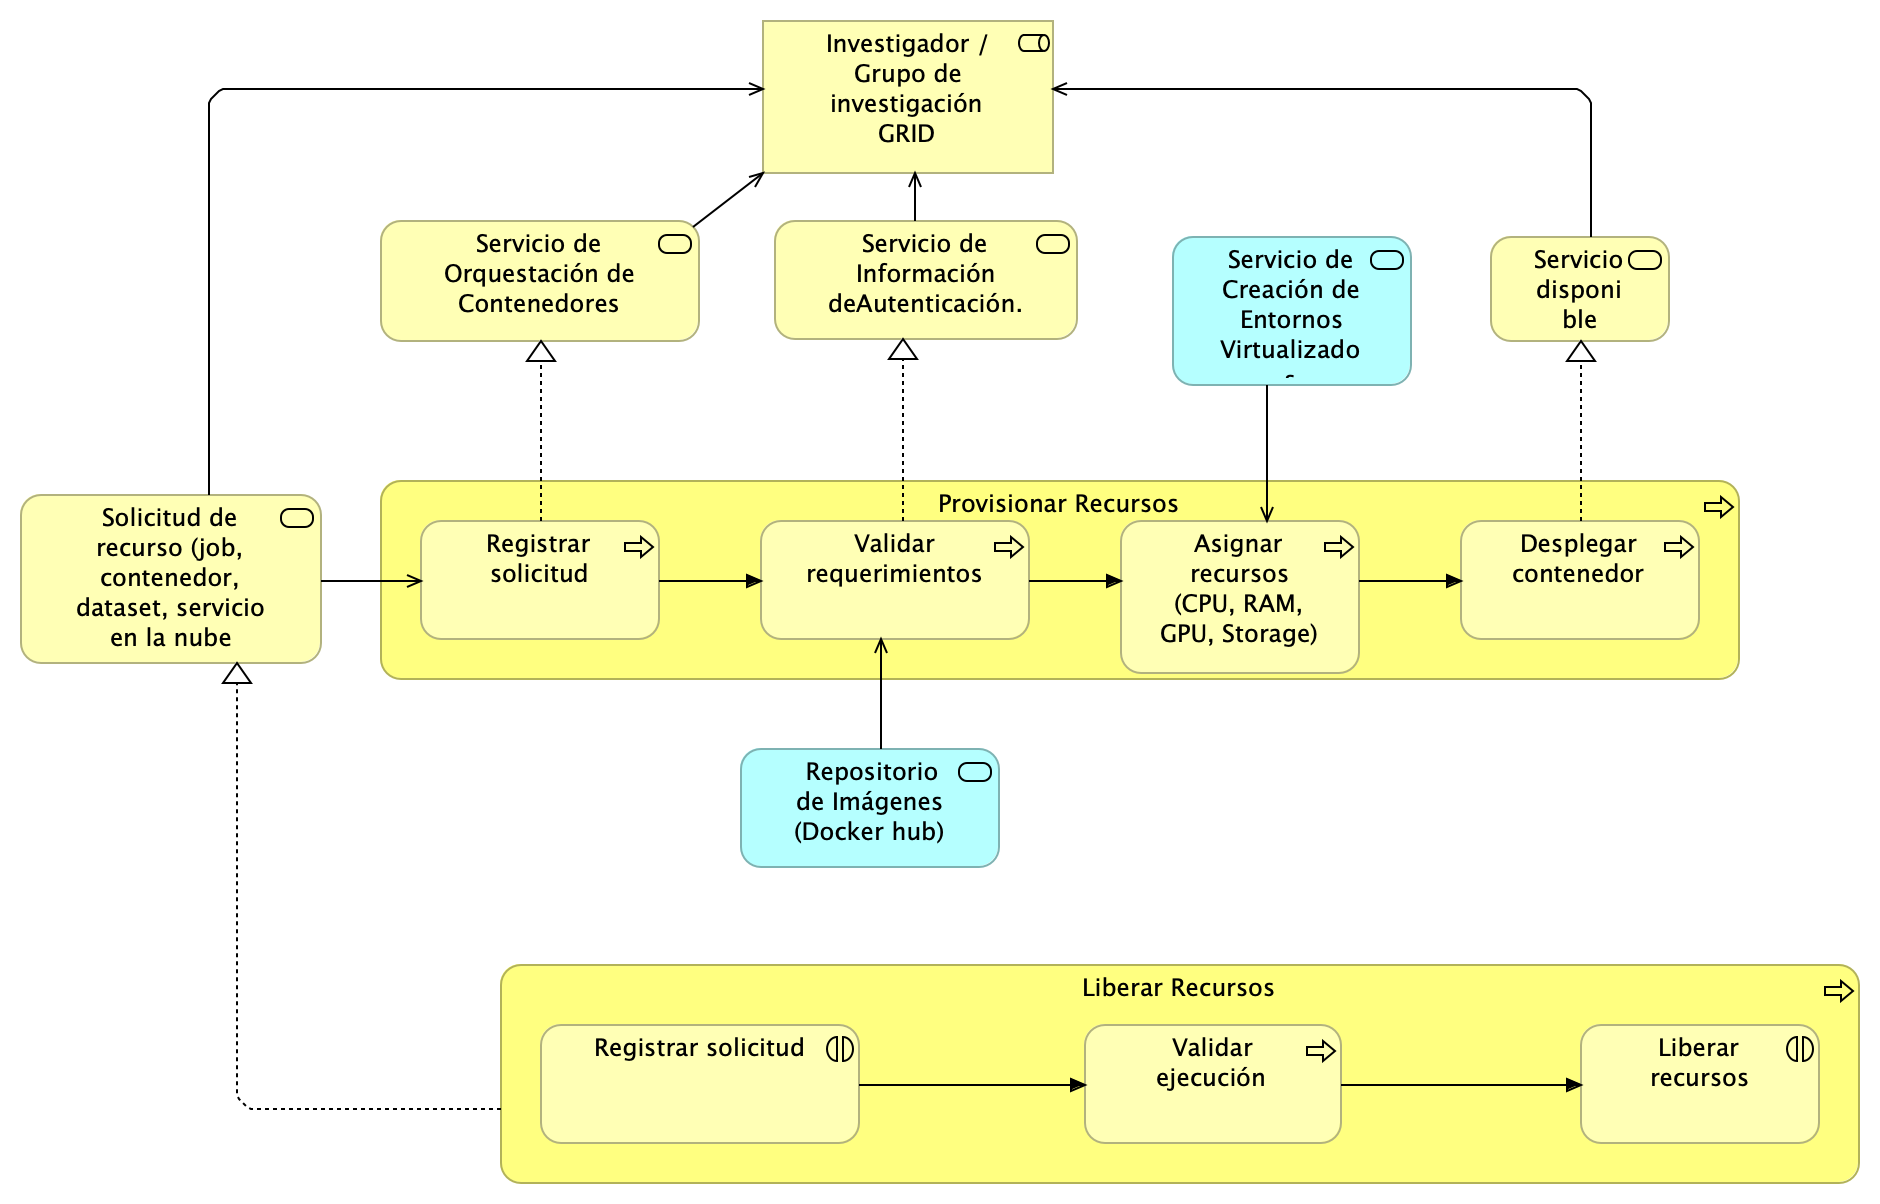
\includegraphics[width=\textwidth]{tablas-images/cp6/Business-Cooperation-View.png}
    \caption{Vista de Cooperación de Negocio}\label{fig:vista-cooperacion-negocio}
\end{figure}
\noindent
El diagrama~\ref{fig:vista-productos-negocio} ilustra cómo los investigadores y estudiantes acceden a los recursos de cómputo bajo un marco regulado por políticas de uso y respaldado por un acuerdo de nivel de nivel de servicio (\SLA, por sus siglas en inglés). Muestra el flujo desde la solicitud hasta la ejecución de los contenedores, buscando la trazabilidad y control en el consumo de infraestructura.

\begin{figure}[H]
    \centering
    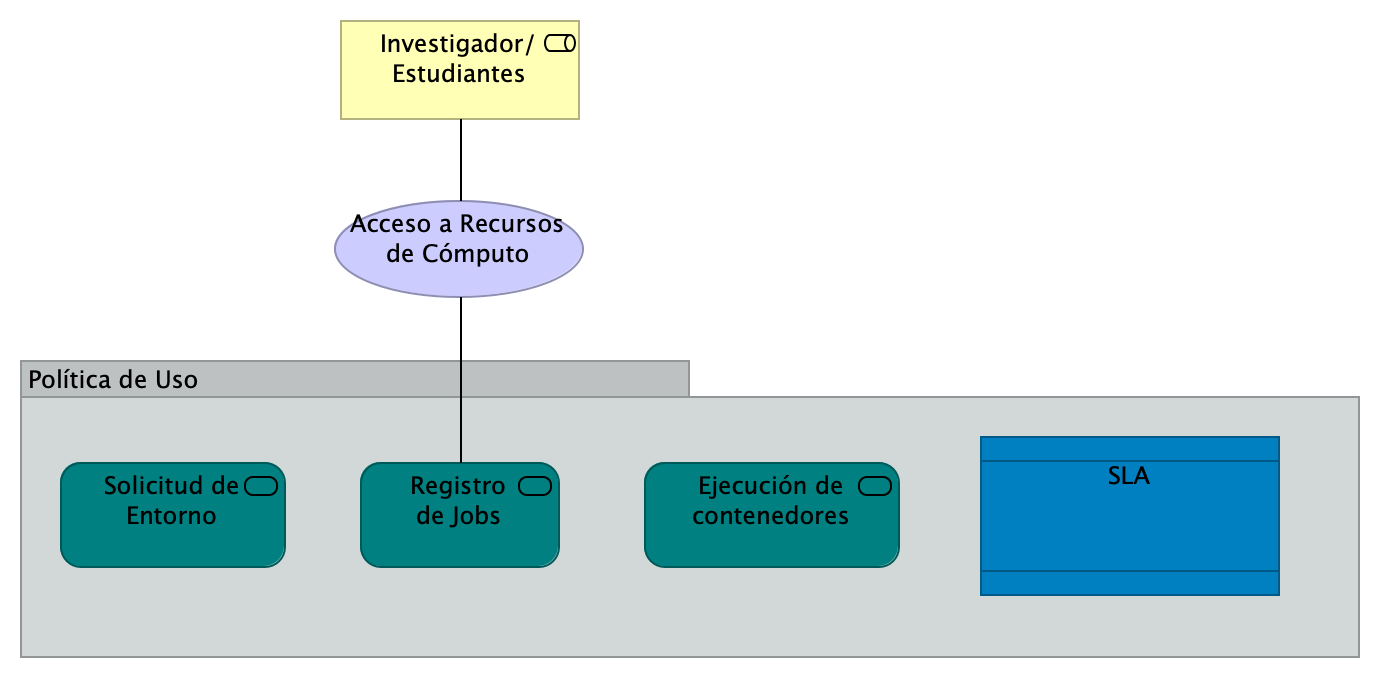
\includegraphics[width=\textwidth]{tablas-images/cp6/Business-Product-View.png}
    \caption{Vista de Producto de Negocio}\label{fig:vista-productos-negocio}
\end{figure}

\noindent
La imagen~\ref{fig:vista-proceso-negocio} muestra el ciclo de vida completo de los entornos de cómputo: desde la solicitud de ejecución por parte de investigadores o estudiantes, pasando por el registro, validación, planificación de recursos y despliegue, hasta la liberación de los recursos una vez usados. En este flujo intervienen componentes clave como descriptores de jobs en Kubernetes, credenciales de clúster, registros de usuario, acuerdos de recursos, autenticación, orquestador y scheduler de prioridad. En conjunto, el modelo refleja cómo se gestionan de manera controlada y auditable los recursos computacionales dentro del sistema.
\begin{figure}[H]
    \centering
    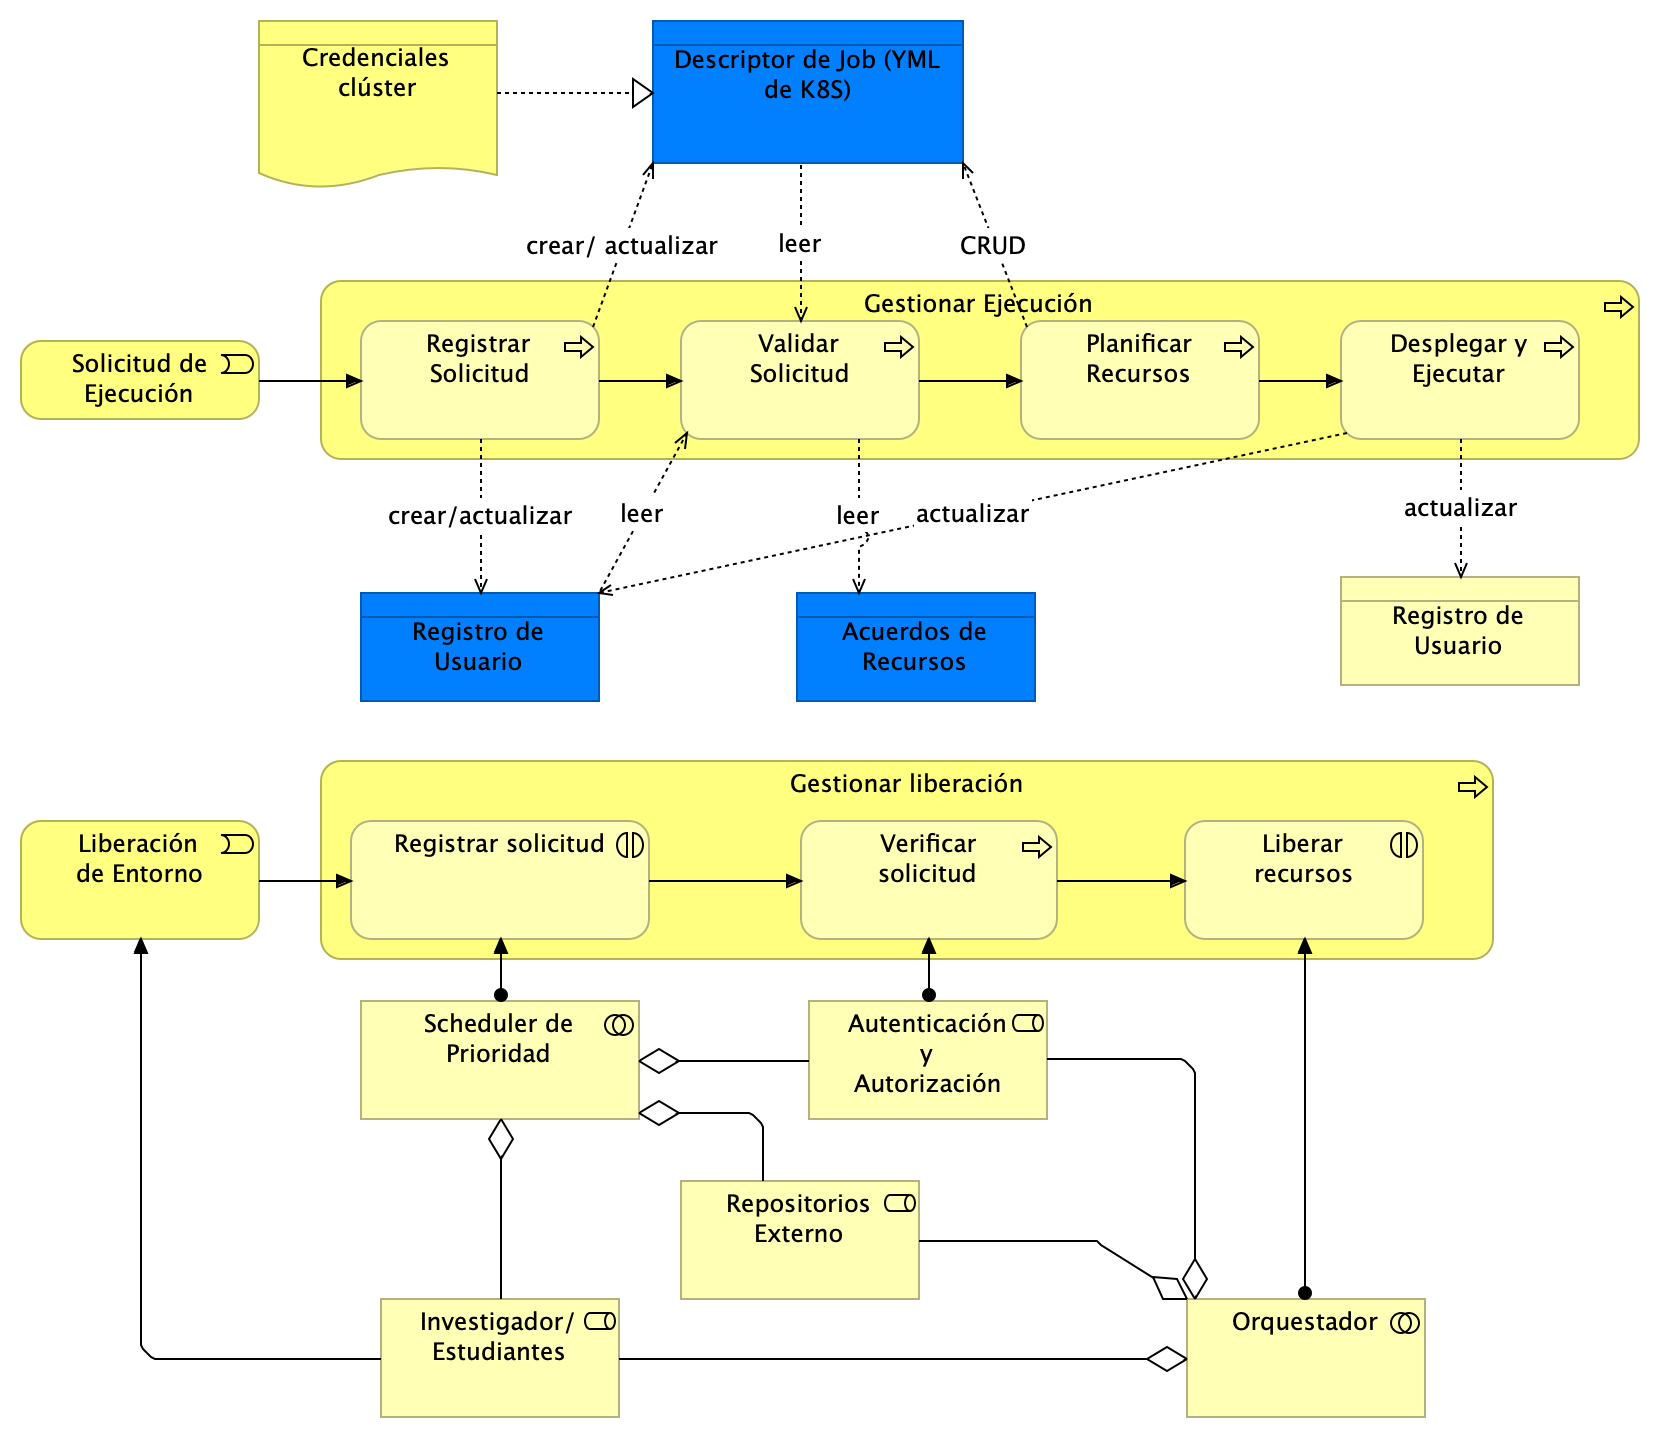
\includegraphics[width=\textwidth]{tablas-images/cp6/Business-Process-View.png}
    \caption{Vista de Proceso de Negocio}\label{fig:vista-proceso-negocio}
\end{figure}
\noindent
El diagrama~\ref{fig:vista-funcion-negocio} muestra cómo la solución de virtualización basada en contenedores del \GRID\ organiza sus principales funciones para dar soporte a estudiantes e investigadores. Entre estas funciones destacan la gestión de colaboraciones externas, la orquestación de recursos, la gestión de infraestructura virtualizada, la gestión de recursos de cómputo y consumo, la gestión de ejecuciones y la gestión de estudiantes e investigadores. El diagrama refleja la interacción entre actores clave, señalando el flujo de información, el uso de infraestructura y los resultados de proyectos, lo que permite una administración alineada con los objetivos académicos y de investigación.

\begin{figure}[H]
    \centering
    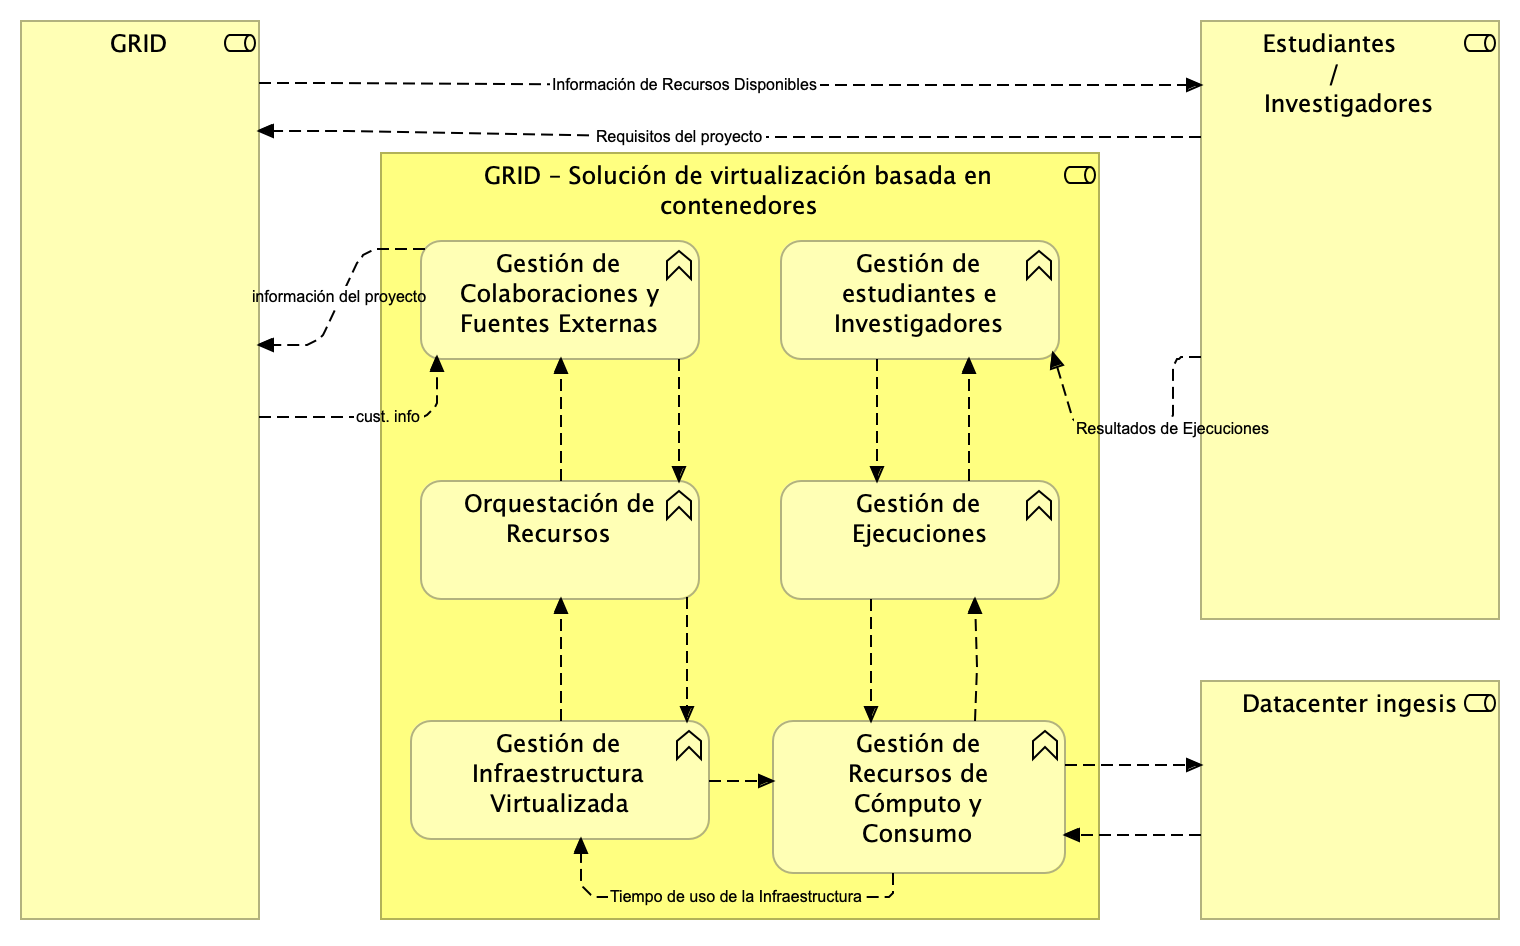
\includegraphics[width=\textwidth]{tablas-images/cp6/Business-Function-View.png}
    \caption{Vista de Función de Negocio}\label{fig:vista-funcion-negocio}
\end{figure}

\subsection{Vista de aplicación}
\noindent
La figura~\ref{fig:vista-cooperacion-aplicacion} muestra la vista de cooperación de aplicaciones, en la cual se representa la interacción entre los componentes de la arquitectura de virtualización y contenerización. En la capa de aplicaciones, se observa el entorno de Containers Applications, conformado por K3S, Containerd, Kubectl y los Pods, que trabajan en conjunto para la gestión y ejecución de contenedores. Estos elementos se relacionan con la infraestructura subyacente compuesta por el hipervisor, las \VM\ y los servicios de almacenamiento, los cuales habilitan los recursos. Asimismo, la red interna del \GRID\ actúa como medio de comunicación entre los distintos componentes, mientras que el \textit{firewall} ofrece un nivel de seguridad adicional al controlar los accesos. Esta vista evidencia la cooperación entre la capa de contenerización y la capa de infraestructura, permitiendo la integración de servicios de red, cómputo y seguridad en un ecosistema unificado.
\begin{figure}[H]
    \centering
    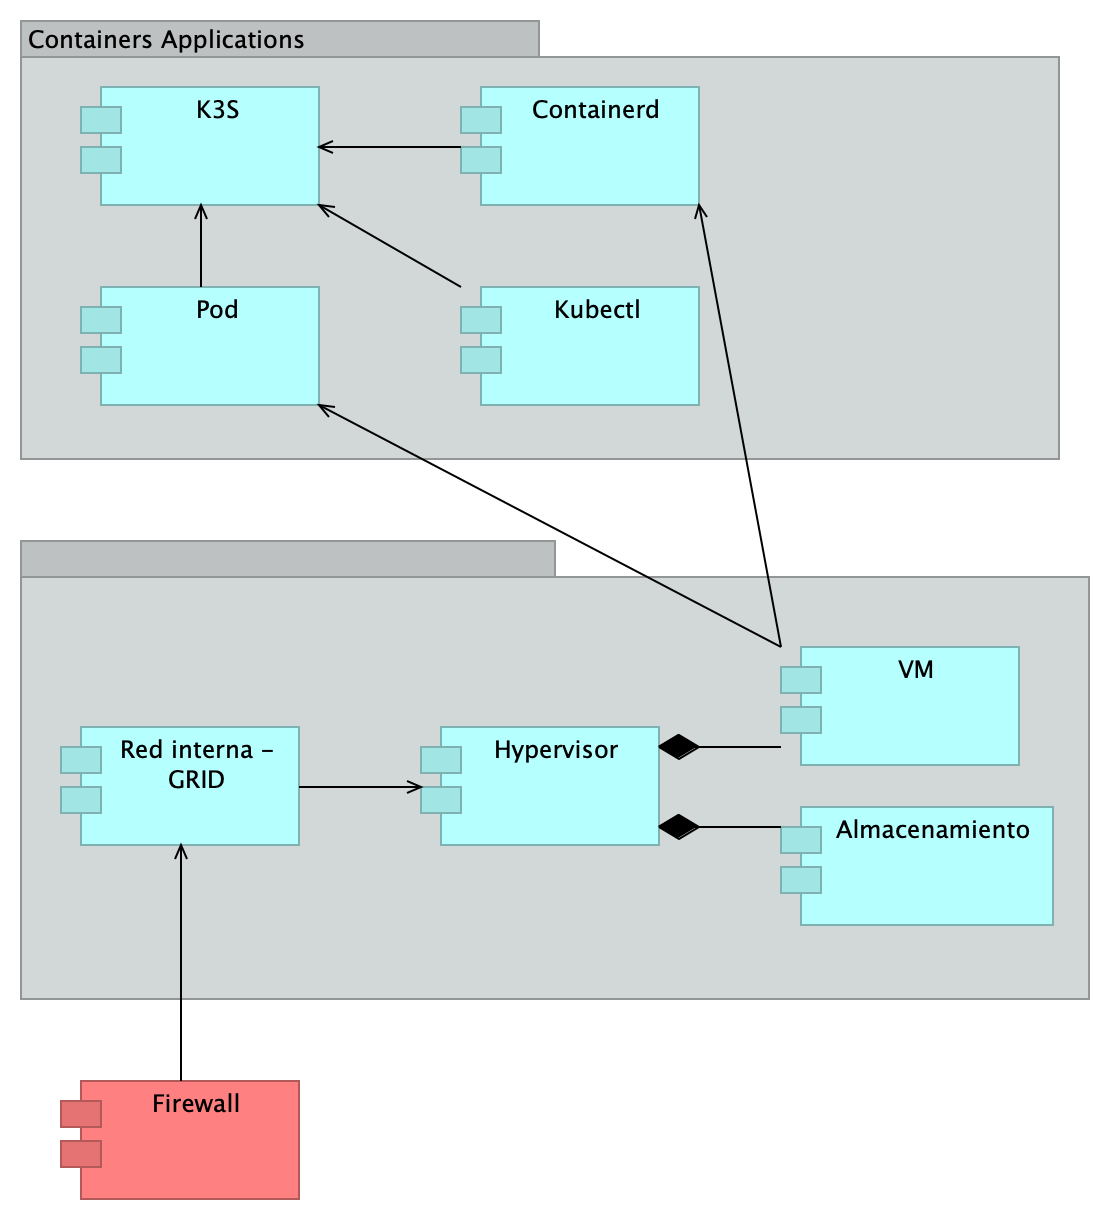
\includegraphics[scale=0.2]{tablas-images/cp6/Application-Cooperation-View.png}
    \caption{Vista de Cooperación de Aplicaciones}\label{fig:vista-cooperacion-aplicacion}
\end{figure}
\noindent
La figura~\ref{fig:vista-comportamiento-aplicacion} presenta la vista de comportamiento de aplicaciones, donde se describe el flujo de actividades relacionadas con la creación automatizada de máquinas virtuales sobre el hipervisor. El proceso inicia con la validación de nombres de las \VM, asociado al parámetro de entrada del número de \textit{workers}, y continúa con la creación del servidor \NAT\ y FailoverNAT, en pro de ofrecer redundancia en la red. Posteriormente, se lleva a cabo la creación de los nodos \textit{master} y \textit{workers}, utilizando como insumo las llaves \SSH\ para la autenticación segura. Finalmente, se realiza la configuración de red, en la cual se definen las direcciones \IP\ y las direcciones \MAC\ de cada nodo. Este comportamiento está agrupado bajo la política de automatización Policy Creation, que organiza de manera estructurada la secuencia de tareas que componen el servicio de creación de \VM, evidenciando cómo los recursos de red, seguridad y cómputo se coordinan para desplegar entornos virtualizados de forma eficiente.
\begin{figure}[H]
    \centering
    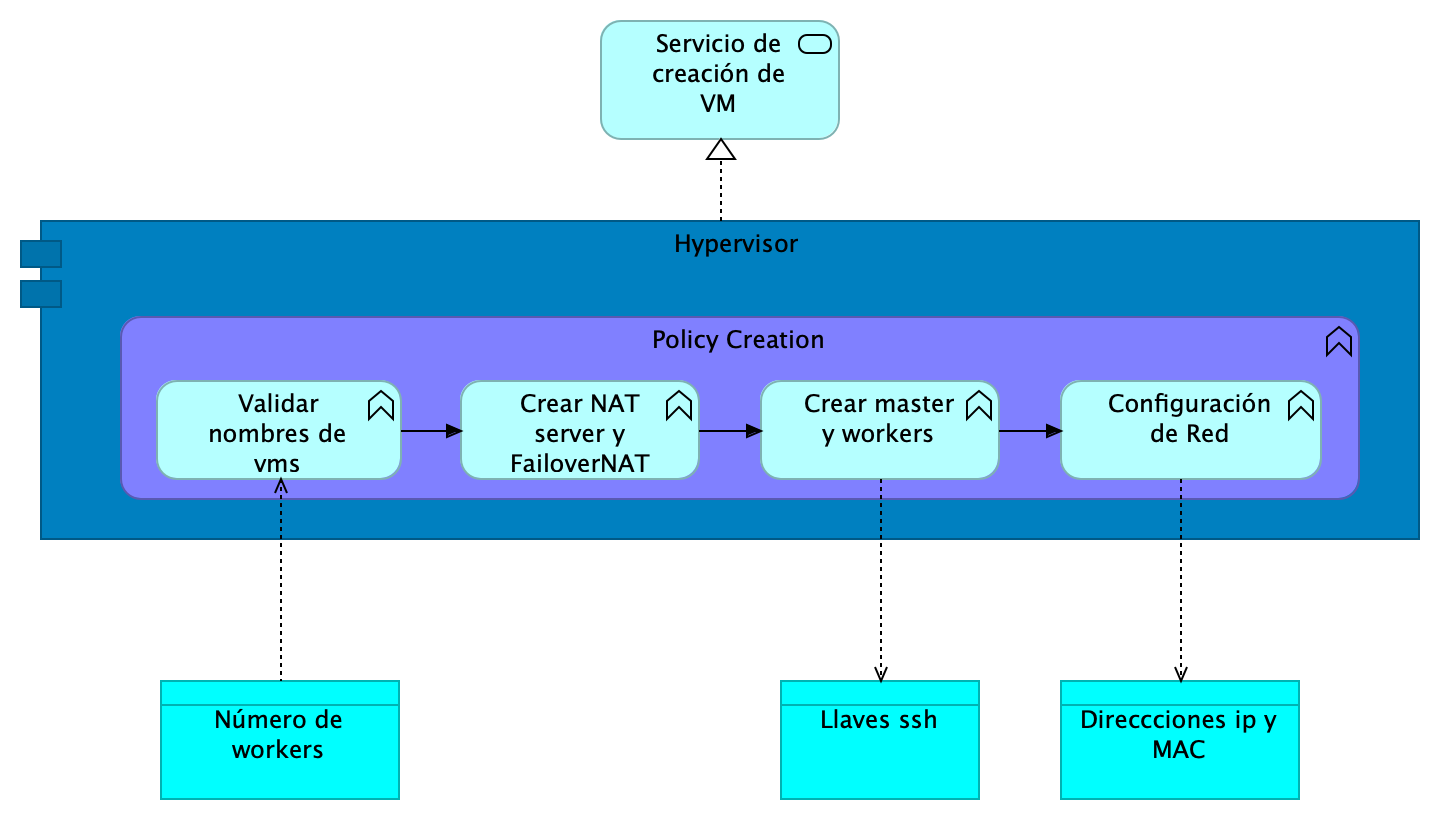
\includegraphics[width=\textwidth]{tablas-images/cp6/Application-Behaviour-view.png}
    \caption{Vista de Comportamiento de Aplicaciones}\label{fig:vista-comportamiento-aplicacion}
\end{figure}
\noindent
El diagrama~\ref{fig:vista-estructura-aplicacion} constituye una vista de estructura de aplicaciones en la cual se modela la organización funcional del sistema de Administración de Recursos del \GRID. En la capa de aplicación, se identifican distintos \textit{Application Components} —como Evaluación de Recursos, Acceso de Investigadores, Gestión de Ejecuciones y Gestión de Entornos Virtualizados— que representan las funcionalidades principales encargadas de articular los procesos del sistema. De este modo, la vista refleja la manera en que los servicios de aplicación soportan la administración de recursos computacionales en el \GRID\ mediante la gestión y persistencia de datos estructurados, buscando la integración entre usuarios, ejecuciones y entornos virtualizados.
\begin{figure}[H]
    \centering
    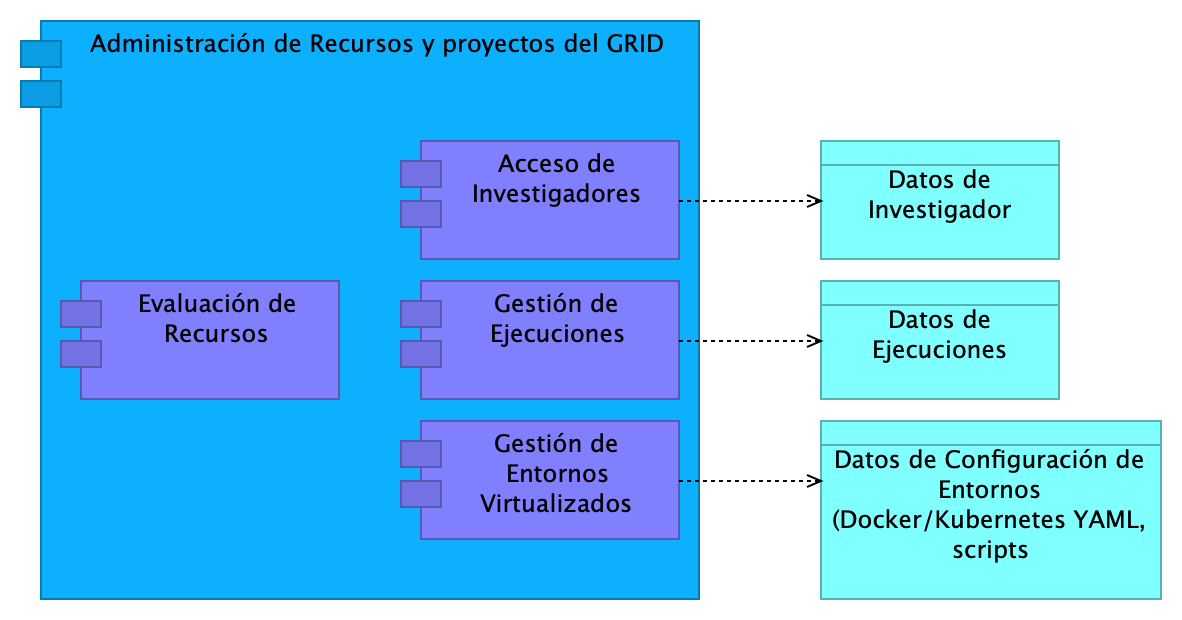
\includegraphics[width=\textwidth]{tablas-images/cp6/Application-Structure-View.png}
    \caption{Vista de Estructura de Aplicaciones}\label{fig:vista-estructura-aplicacion}
\end{figure}

\subsection{Vista de tecnología}
\begin{figure}[H]
    \centering
    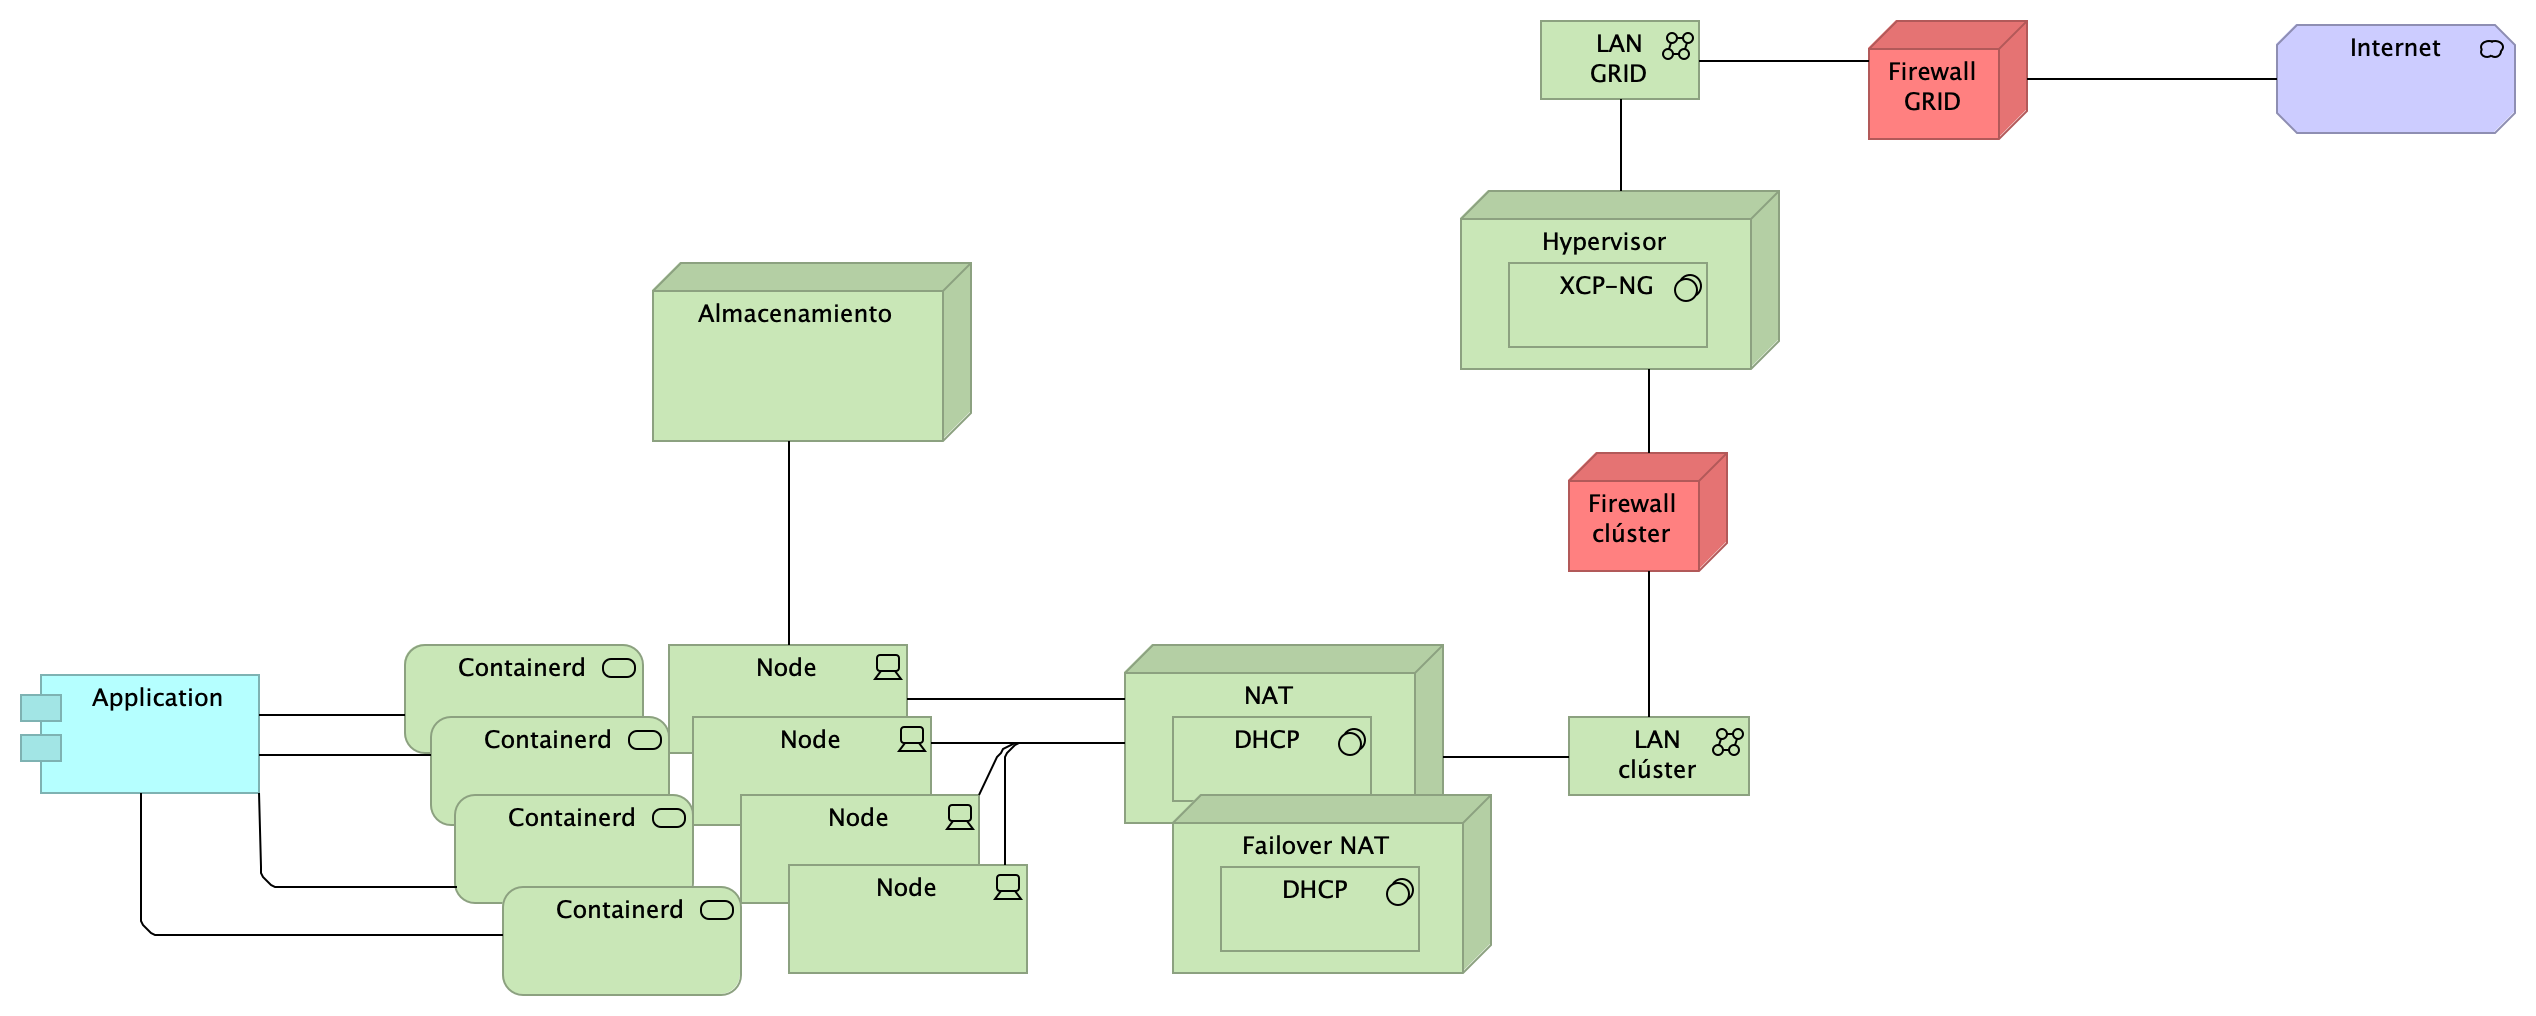
\includegraphics[width=\textwidth]{tablas-images/cp6/Implementation-and-Installation-View.png}
    \caption{Vista de Implementación e Instalación}
\end{figure}
\begin{figure}[H]
    \centering
    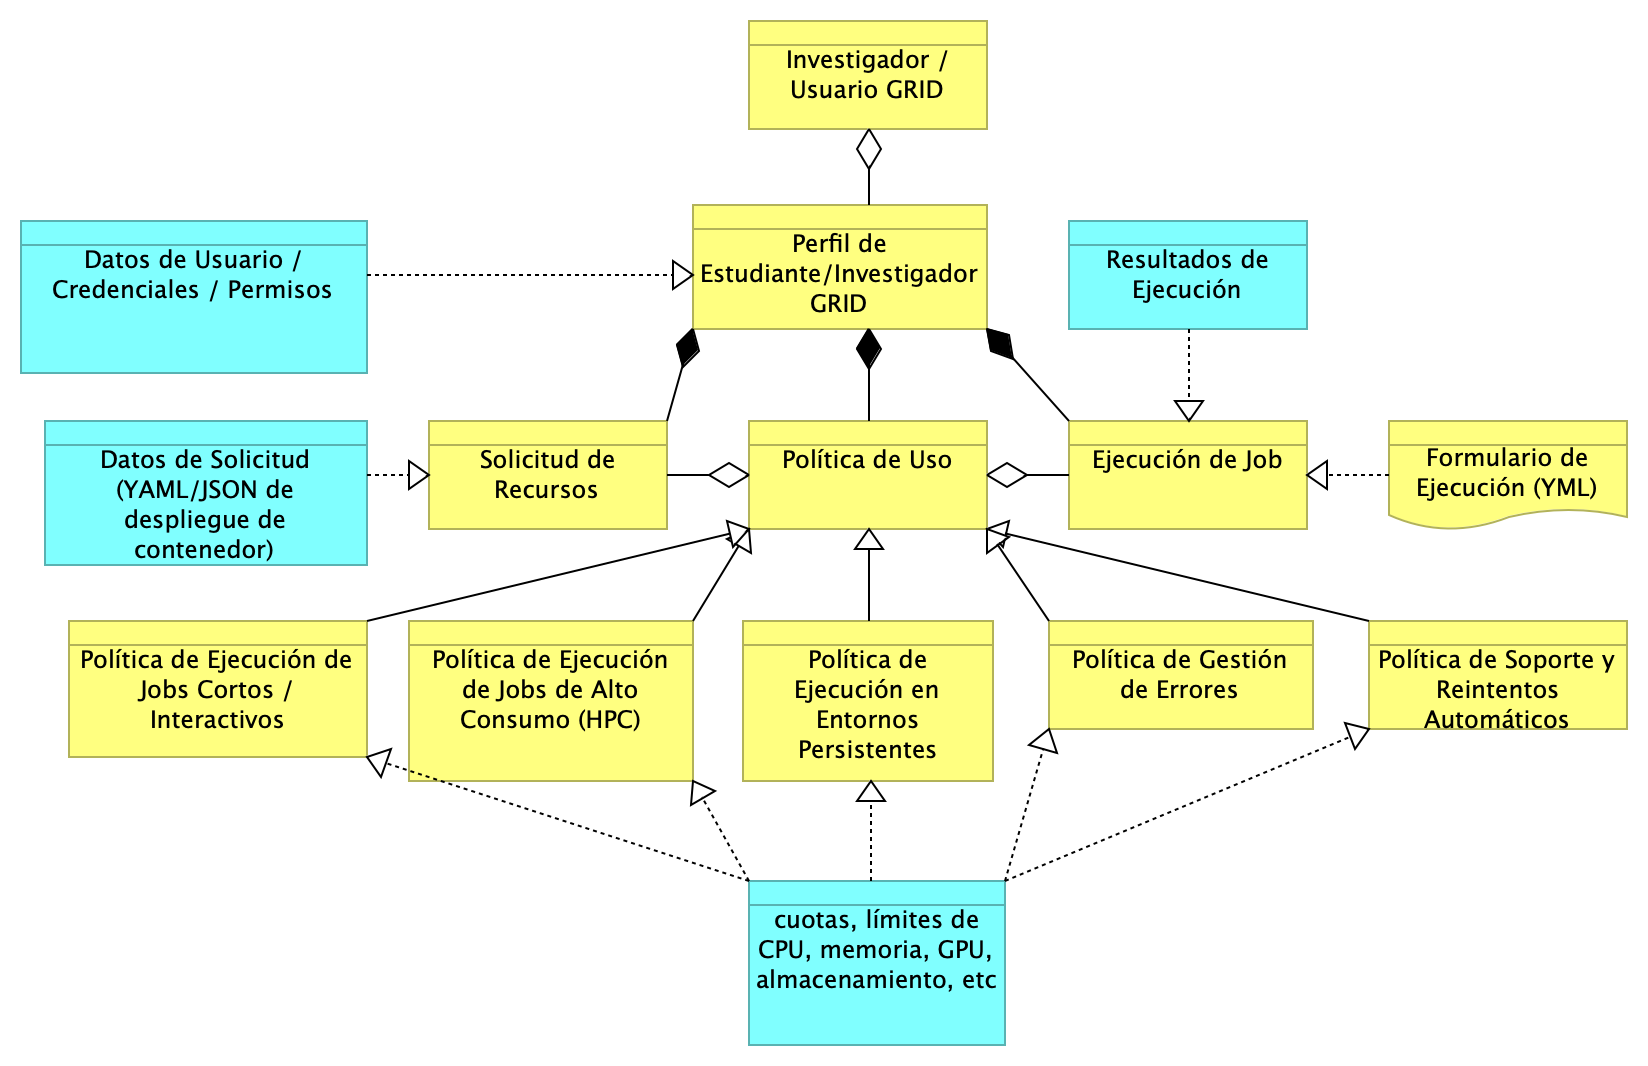
\includegraphics[width=\textwidth]{tablas-images/cp6/Information-Structure-View.png}
    \caption{Vista de Estructura de Información}
\end{figure}x


\subsection{Vista general}
\begin{figure}[H]
    \centering
    \input{tablas-images/cp6/Layered-View.png}
\end{figure}

\section{Diseño por capas de la solución}

\section{Capa de infraestructura}

\begin{figure}[H]
    \centering
    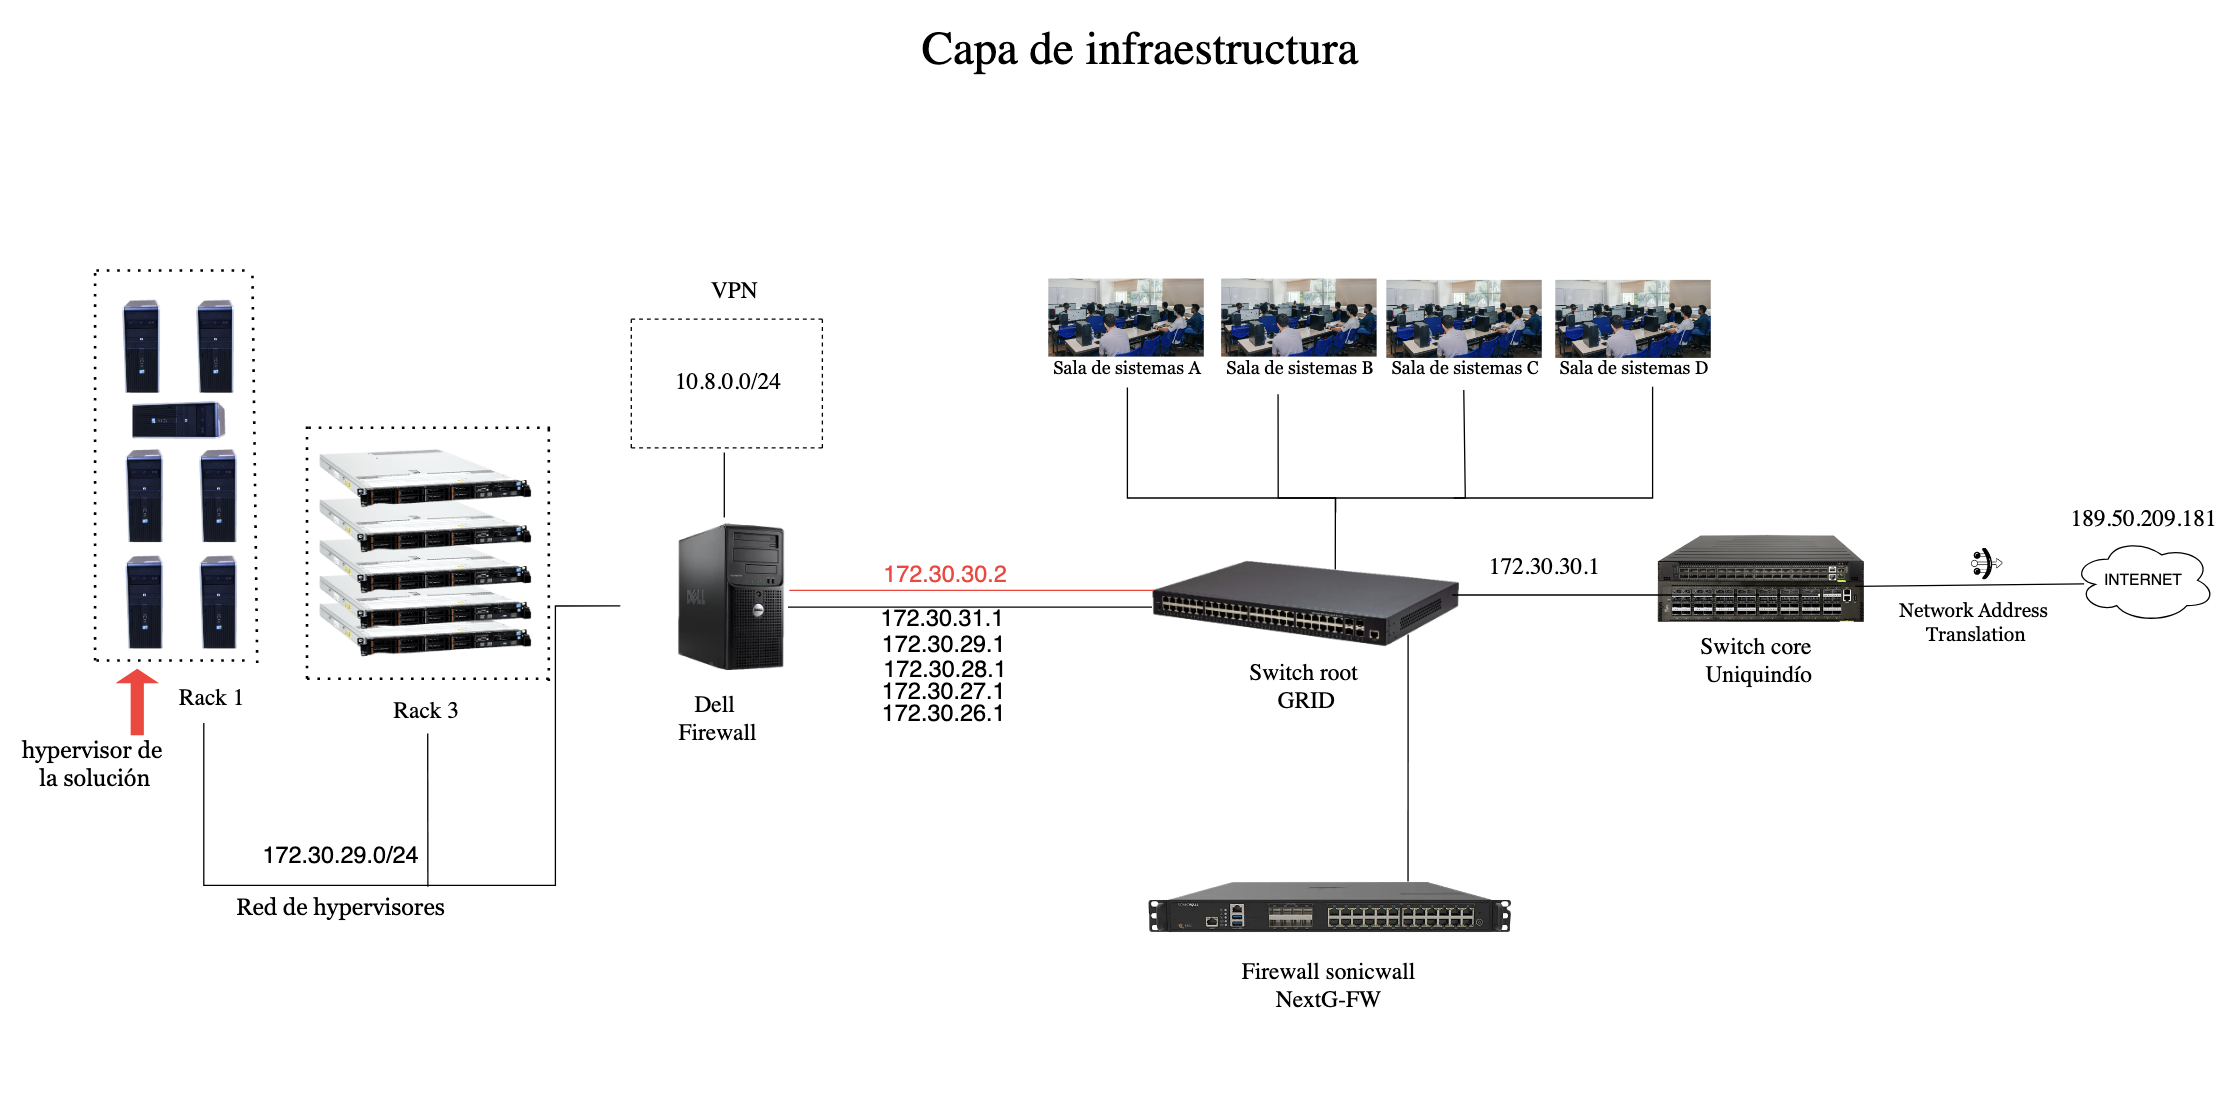
\includegraphics[width=\textwidth]{tablas-images/cp6/disenio-N1.png}
    \caption{Capa de Infraestructura}
\end{figure}

\section{Capa de virtualización}

\begin{figure}[H]
    \centering
    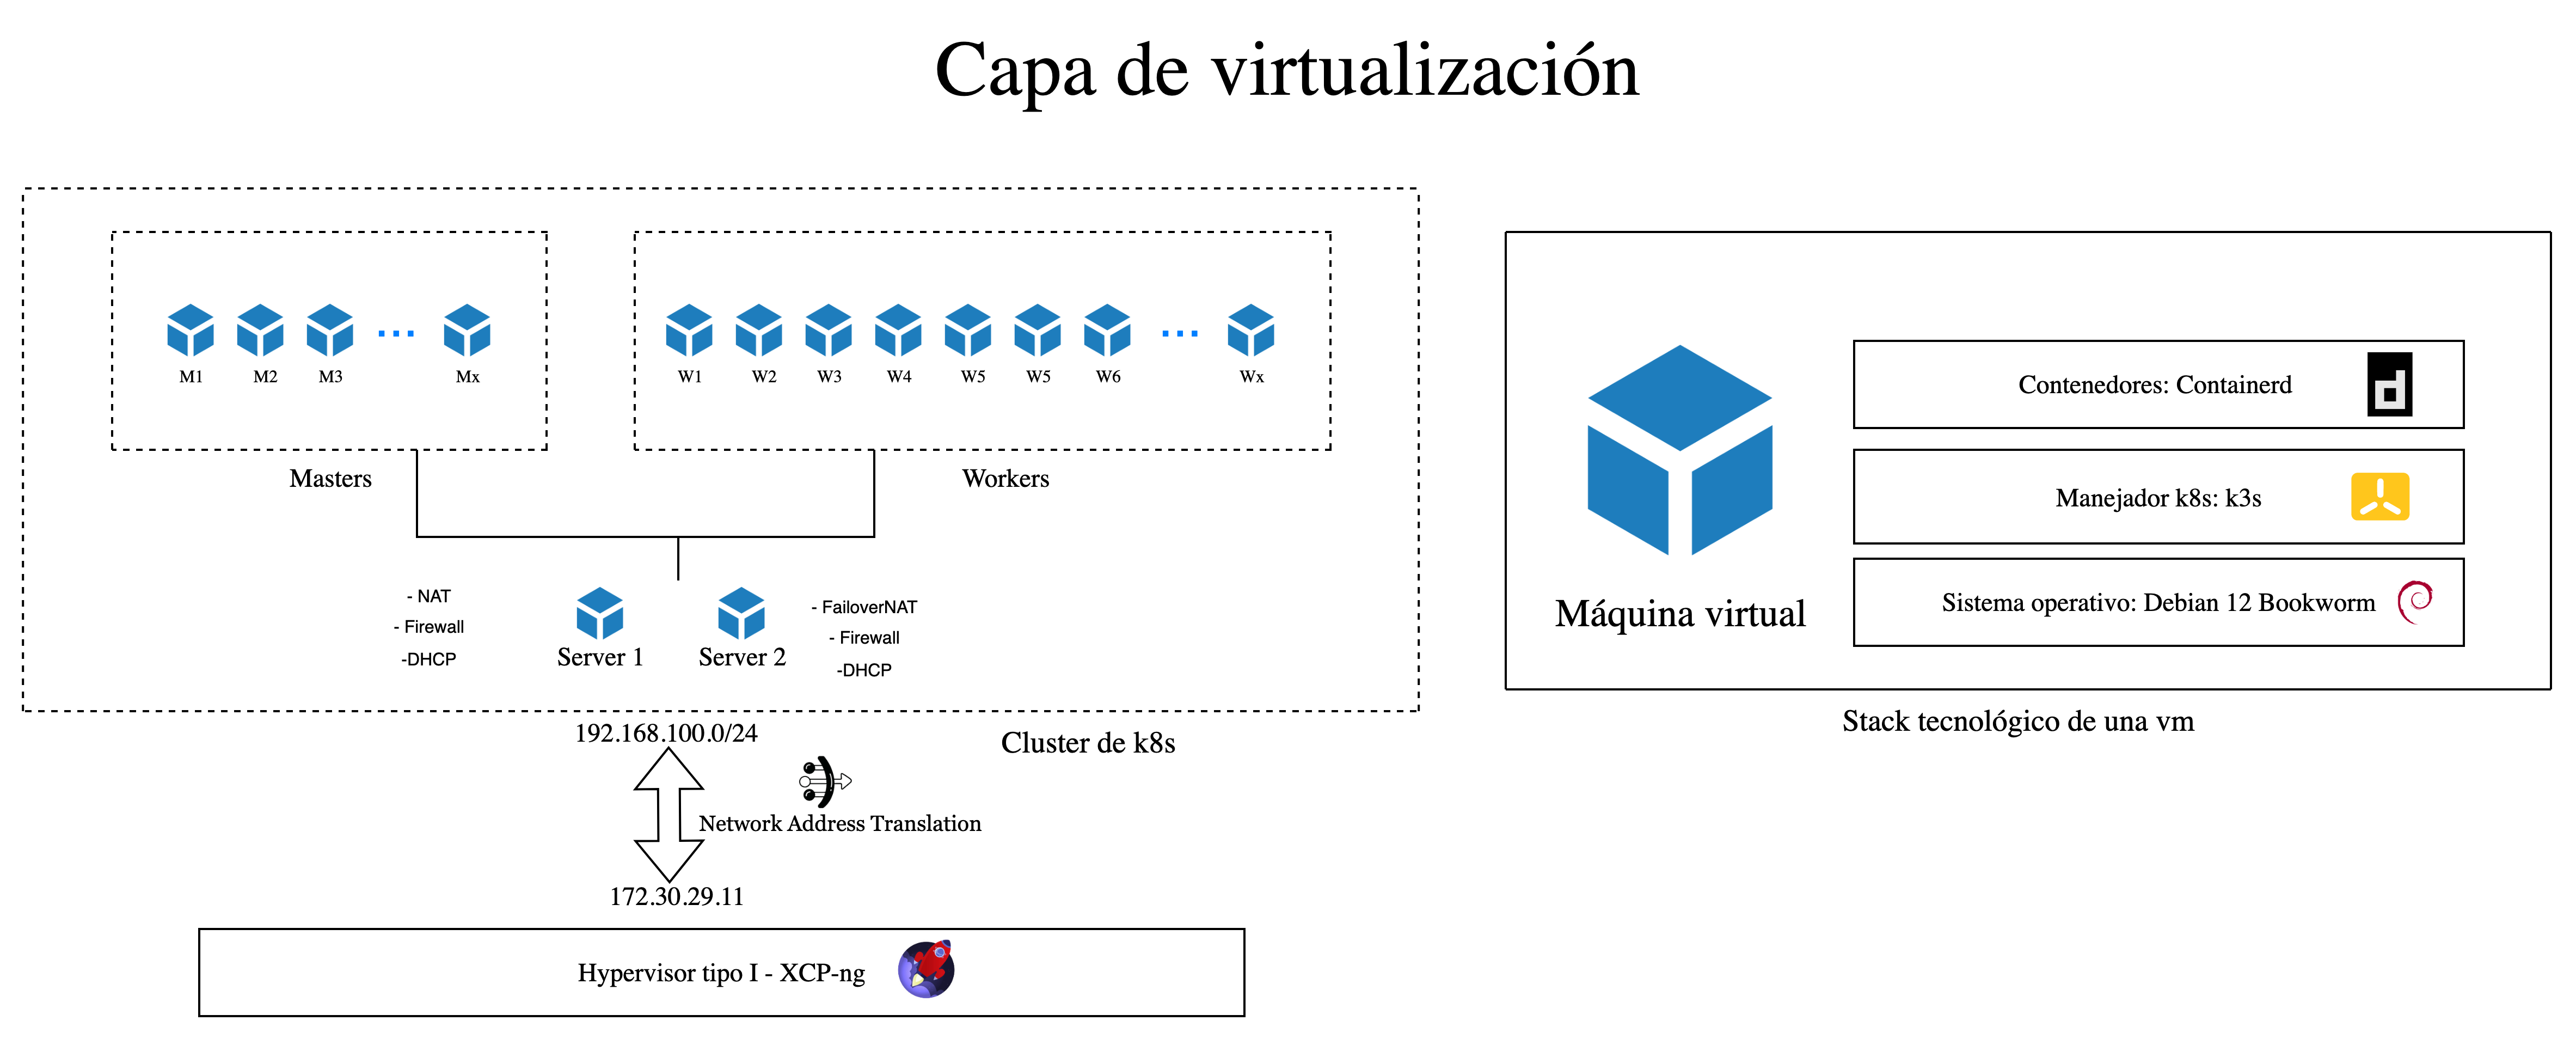
\includegraphics[width=\textwidth]{tablas-images/cp6/disenio-N2.png}
    \caption{Capa de Virtualización}
\end{figure}

\section{Capa de aplicación}
